\documentclass[../main.tex]{subfiles}
\graphicspath{{\subfix{../images/}}} % Images path

\begin{document}

\section{Appendix}\label{appendix}

\subsection{Descriptors Distribution}\label{app:keypoints-distribution}

\begin{figure}[htb]
  \centering
  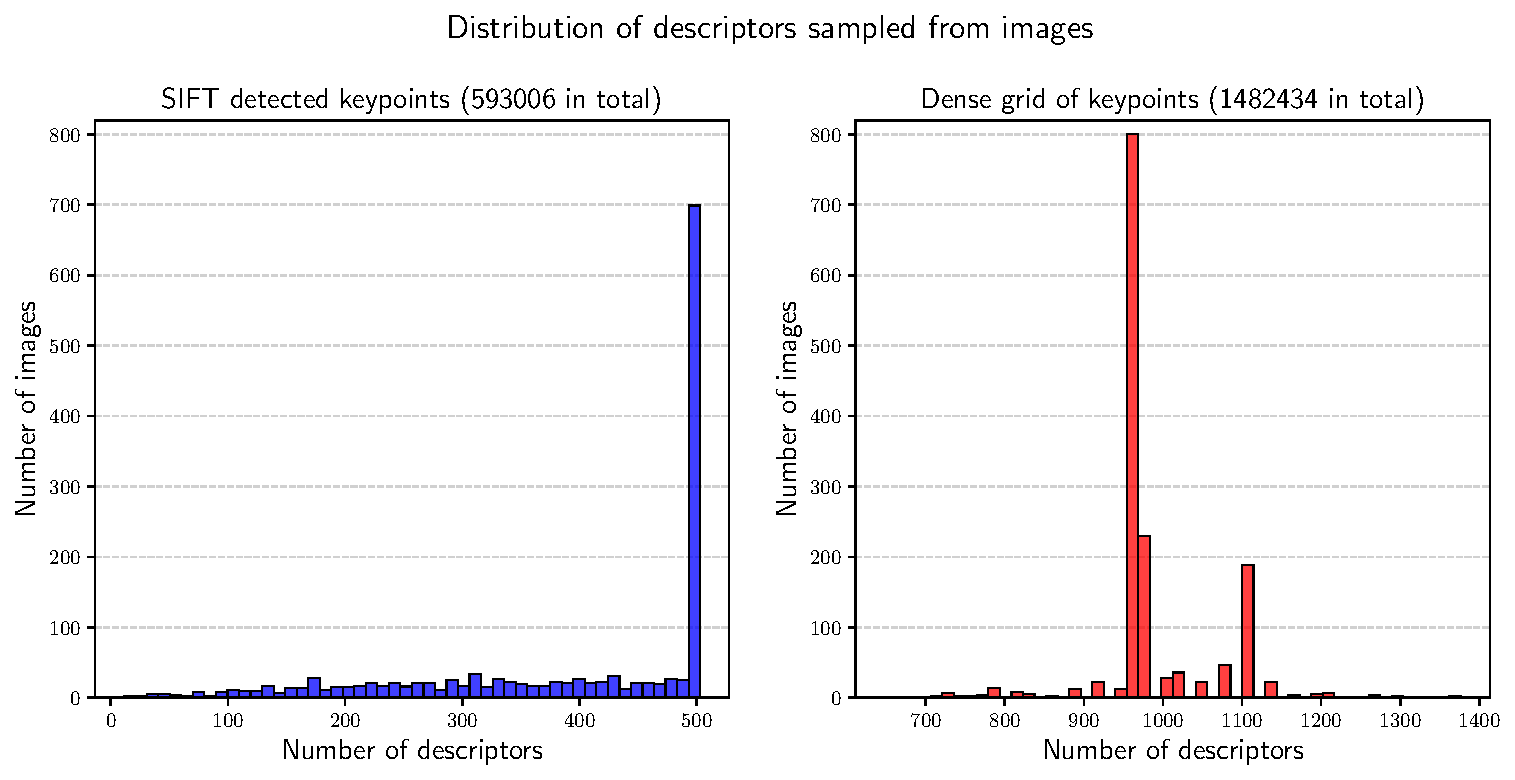
\includegraphics[width=\textwidth]{descriptors_distribution.pdf}
  \caption{Distribution of keypoints sampled from the train set using the SIFT
  detector (\itt{blue}) and the dense grid approach (\itt{red}). For the first
  method, the desired number of keypoints ($500$) has been detected in the
  majority of the images, while for the second method the number of keypoints
  per image is concentrated around $1000$ with small differences due to the
  different sizes and aspect ratios of the images.}\label{fig:keypoints-distribution}
\end{figure}

\subsection{Kernel Density Estimation}\label{app:kernel-density-estimation}

The Gaussian density estimator $K_{\sigma}(x)$ is defined as
\begin{equation}
  K_{\sigma}(x) = \frac{1}{\sqrt{2\pi}\sigma} \exp\left(-\frac{x^2}{2\sigma^2}\right)
\end{equation}

Whereas, given the fact that both visual words and SIFT descriptors are
$128$-dimensional vectors, the Euclidean distance $D(w_i, x_j)$ between the $i$-th visual word $w_i$ and the $j$-th descriptor $x_j$ can be introduced as
\begin{equation}
  D(w_i, x_j) = ||w_i - x_j|| = \sqrt{\sum_{k=1}^{128} (w_{ik} - x_{jk})^2}
\end{equation}

Hence the soft assignment approach proposed by \itt{Van Gemert et
al.}~\cite{gemert} relies on the density estimator
\begin{equation}
  K_{\sigma}(D(w_i, x_j)) = \frac{1}{\sqrt{2\pi}\sigma} \exp\left(-\frac{D(w_i, x_j)^2}{2\sigma^2}\right)
\end{equation}

\pagebreak
\subsection{Confusion Matrices}\label{app:confusion-matrices}

Here the confusion matrices for all the classifiers are reported. These matrices
refer to the case in which features have been extracted by a SIFT descriptor
from keypoints sampled on a dense grid on the images and the input
representation is the normalized histograms of visual words (\itt{HIST}). This has been done to maintain the results consistent with the ones obtained using the spatial pyramid matching approach and to be able to compare the performances of the different classifiers. However, similar matrices can be computed in the other cases as well.\\

\begin{figure}[htb]
  \centering
  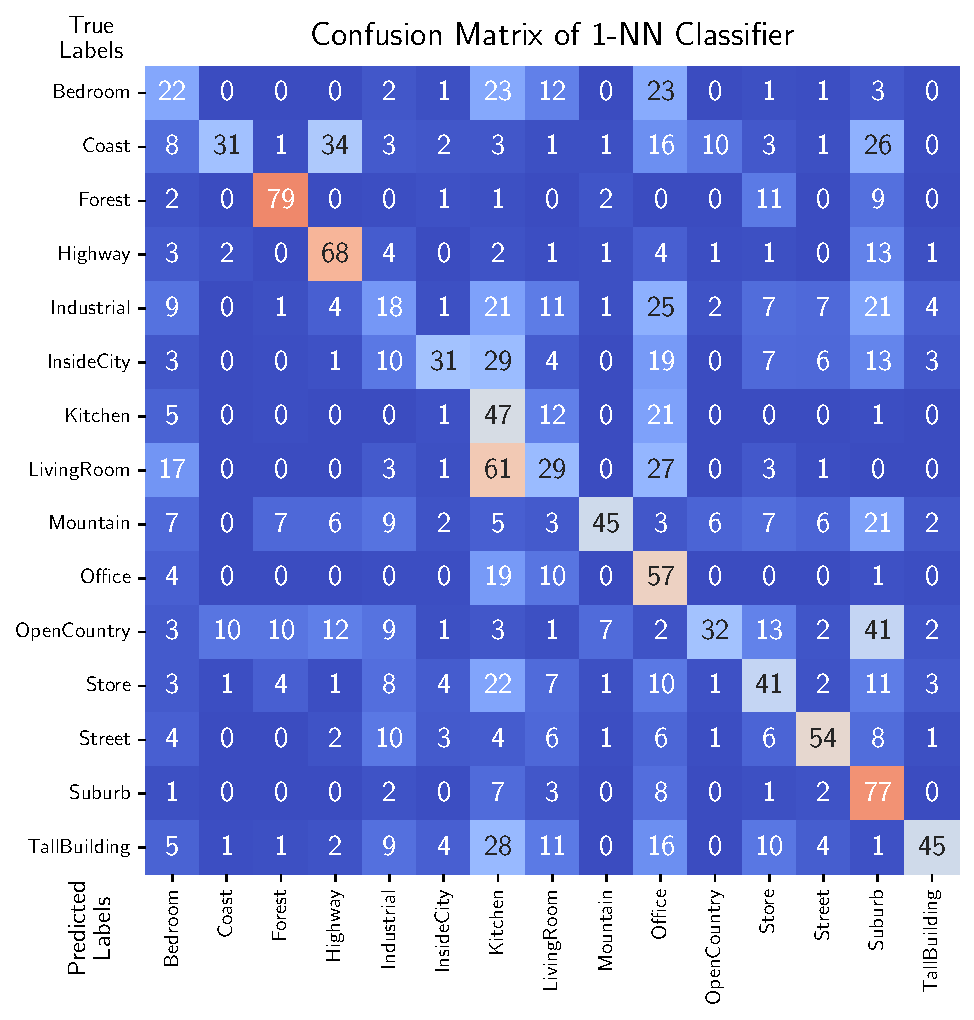
\includegraphics[width=0.8\textwidth]{1nn_confusion_matrix.pdf}
  \caption{Confusion matrix for the 1-NN classifier.}\label{fig:confusion-matrix-1nn}
\end{figure}

\begin{figure}[htb]
  \centering
  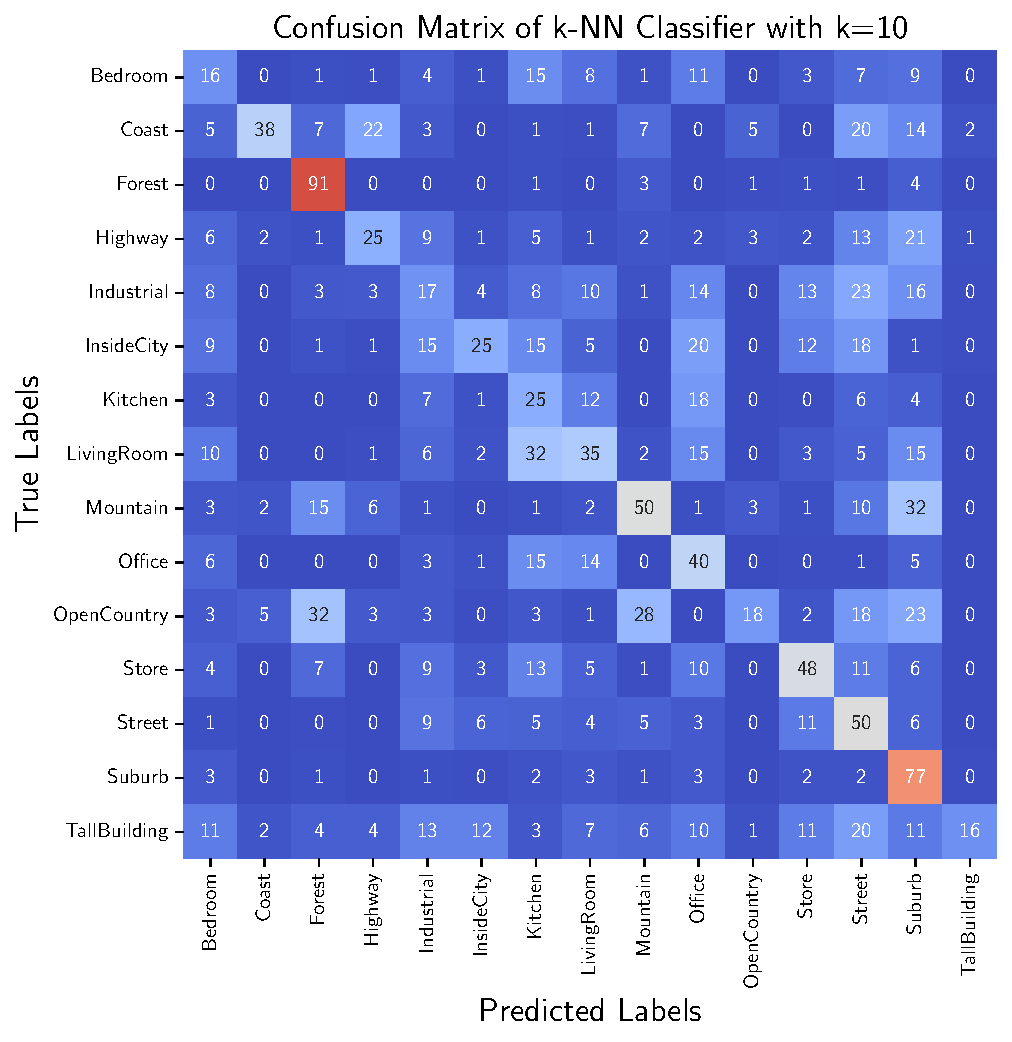
\includegraphics[width=0.8\textwidth]{knn_confusion_matrix.pdf}
  \caption{Confusion matrix for the k-NN classifier with $k = 5$.}\label{fig:confusion-matrix-knn}
\end{figure}

\begin{figure}[htb]
  \centering
  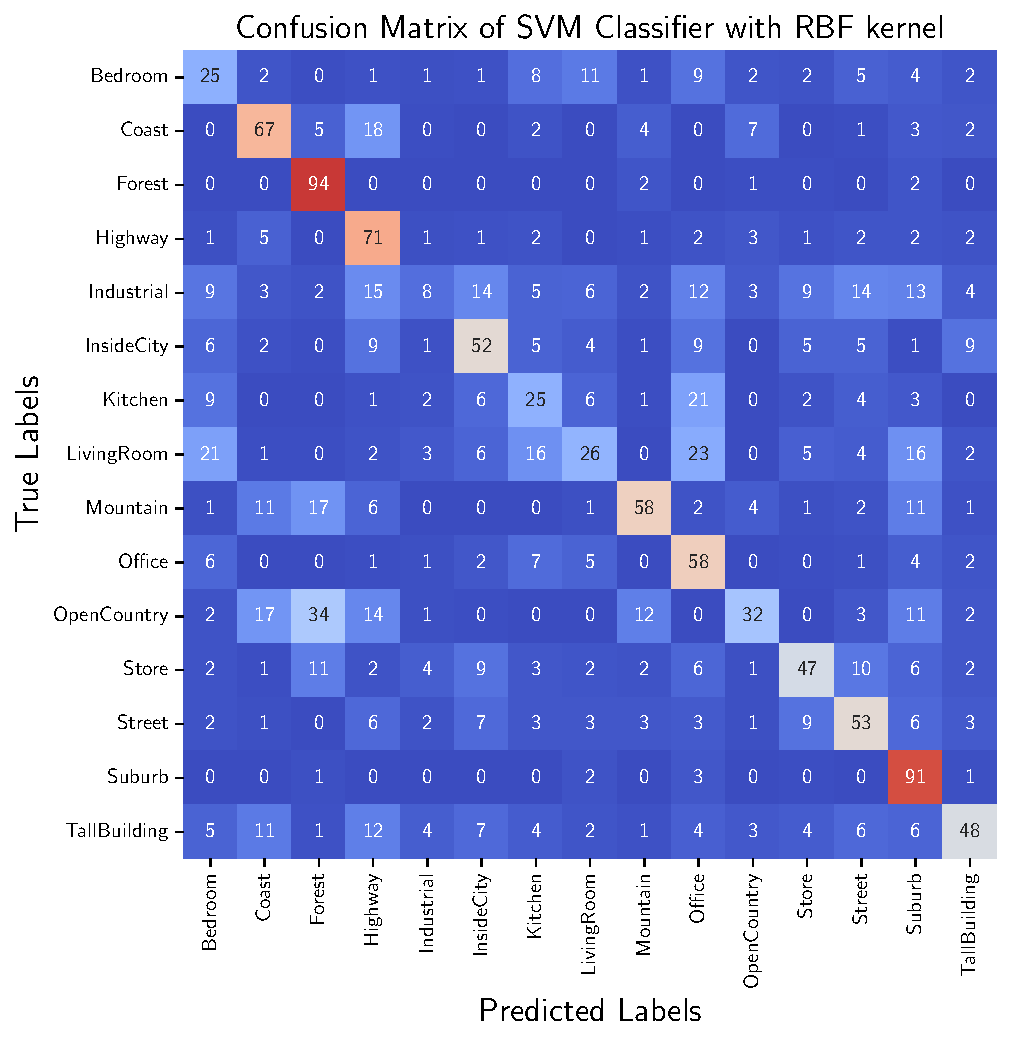
\includegraphics[width=0.8\textwidth]{svm_rbf_confusion_matrix.pdf}
  \caption{Confusion matrix for the SVM classifier with RBF kernel.}\label{fig:confusion-matrix-rbf}
\end{figure}

\begin{figure}[htb]
  \centering
  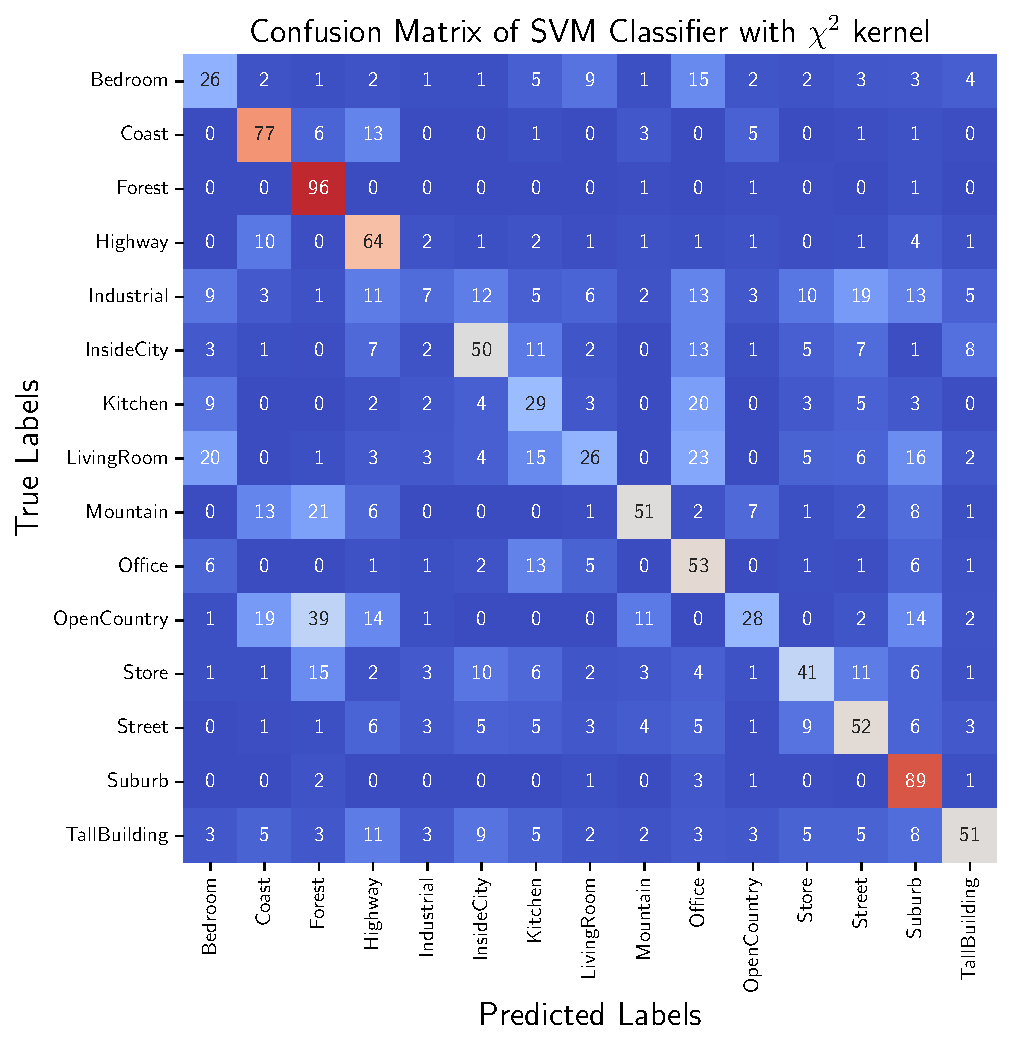
\includegraphics[width=0.8\textwidth]{svm_chi2_confusion_matrix.pdf}
  \caption{Confusion matrix for the SVM classifier with $\chi^2$ kernel.}\label{fig:confusion-matrix-chi2}
\end{figure}

\begin{figure}[htb]
  \centering
  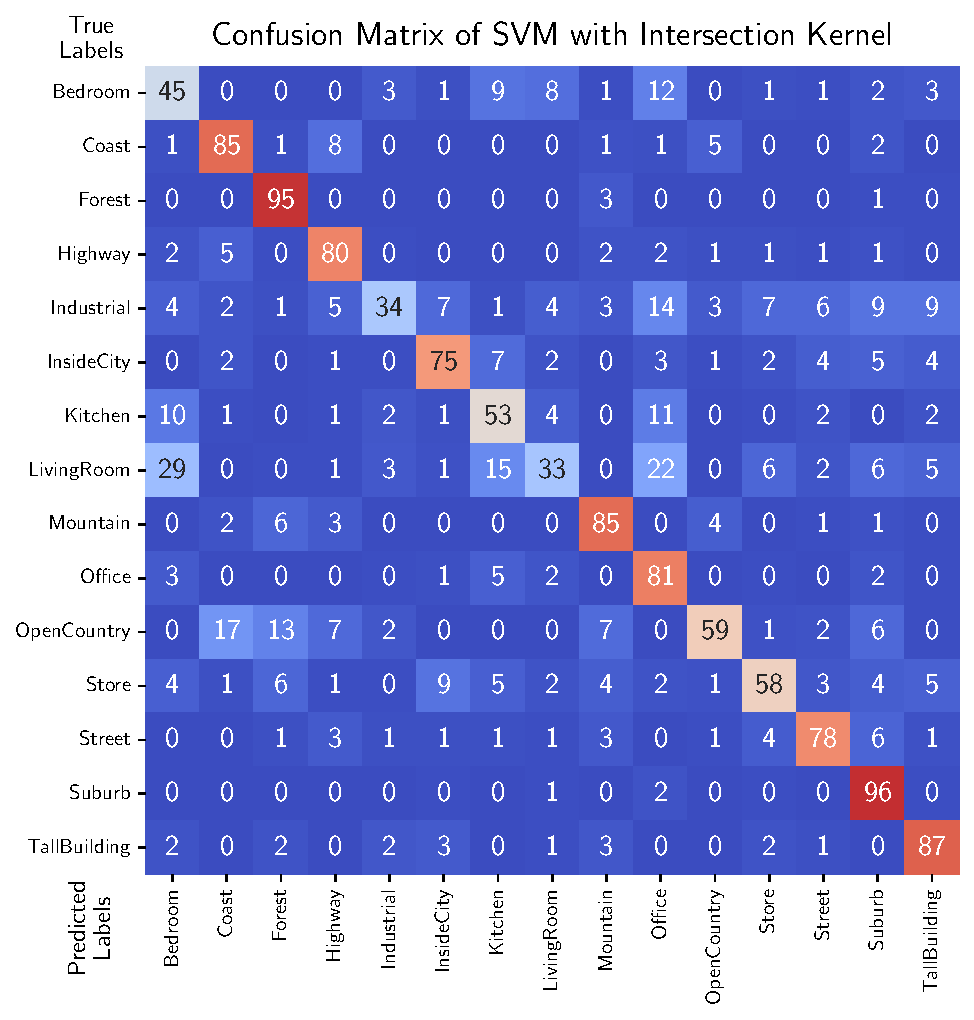
\includegraphics[width=0.8\textwidth]{svm_intersection_confusion_matrix.pdf}
  \caption{Confusion matrix for the SVM classifier with histogram intersection kernel.}\label{fig:confusion-matrix-intersection}
\end{figure}

\FloatBarrier

\begin{figure}[htb]
  \centering
  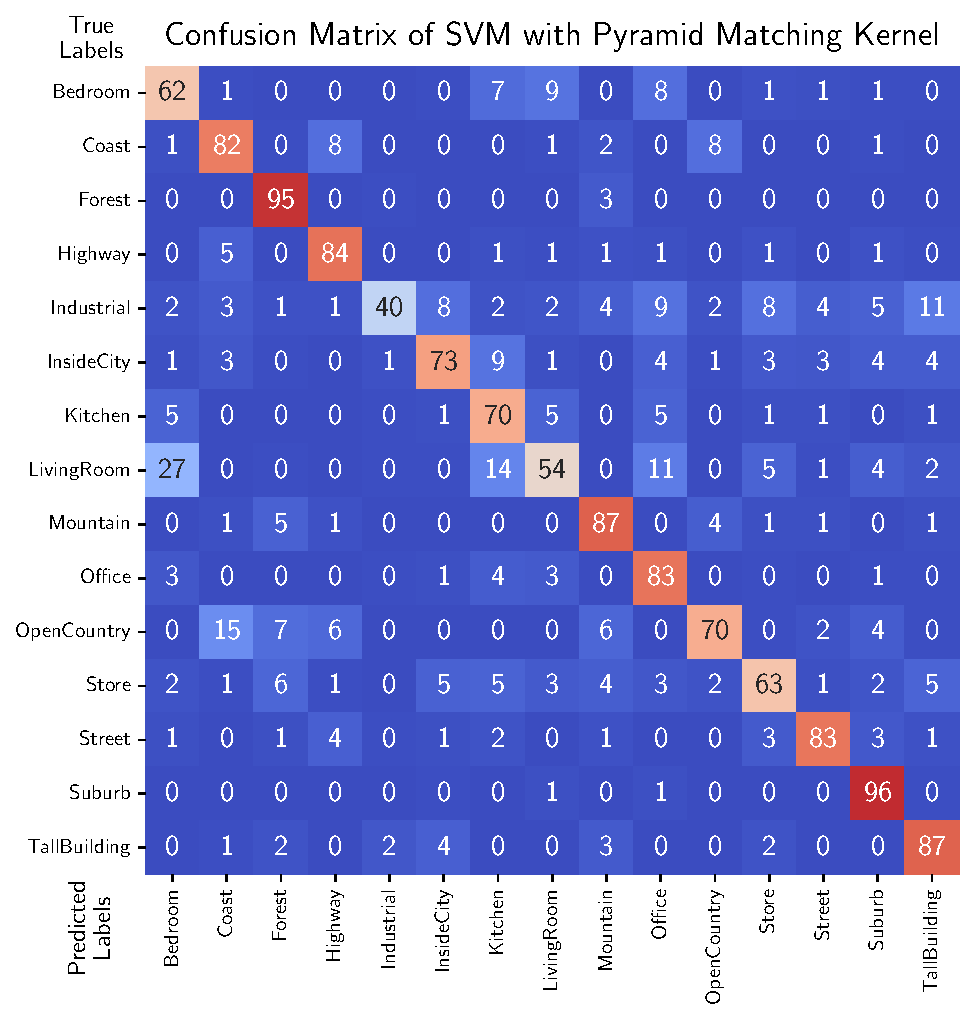
\includegraphics[width=0.8\textwidth]{svm_pyramid_confusion_matrix.pdf}
  \caption{Confusion matrix for the SVM classifier with spatial pyramid matching
  approach.}\label{fig:confusion-matrix-pmk}
\end{figure}


\subsection{Notice on Generative Tools Usage}\label{app:generative-tools}

Generative AI tools have been used as a support for the development of this
project. In particular, the
\href{https://en.wikipedia.org/wiki/Microsoft_Copilot}{Copilot \faLink} generative tool
based on \href{https://en.wikipedia.org/wiki/GPT-4}{OpenAI GPT 4o \faLink} model has
been used as assistance medium in performing the following tasks:

\begin{itemize}
	 \item writing documentation and comments in implemented functions by
		 adhering to the
		 \href{https://numpydoc.readthedocs.io/en/latest/format.html}{NumPy
		 Style Guide \faLink}

	\item improving variable naming and code readability 
	
	\item minor bug fixing in implemented functions

	\item grammar and spelling check both in the repository
		\ttt{README}~\cite{github} and in this report

	\item tweaking aesthetic improvements in the plots of this report

	\item formatting table of results in this report
\end{itemize}

\end{document}


